\chapter*{Sommario} % senza numerazione
\label{sommario}

\addcontentsline{toc}{chapter}{Sommario} % da aggiungere comunque all'indice

\begin{figure}[h]
  \centering
  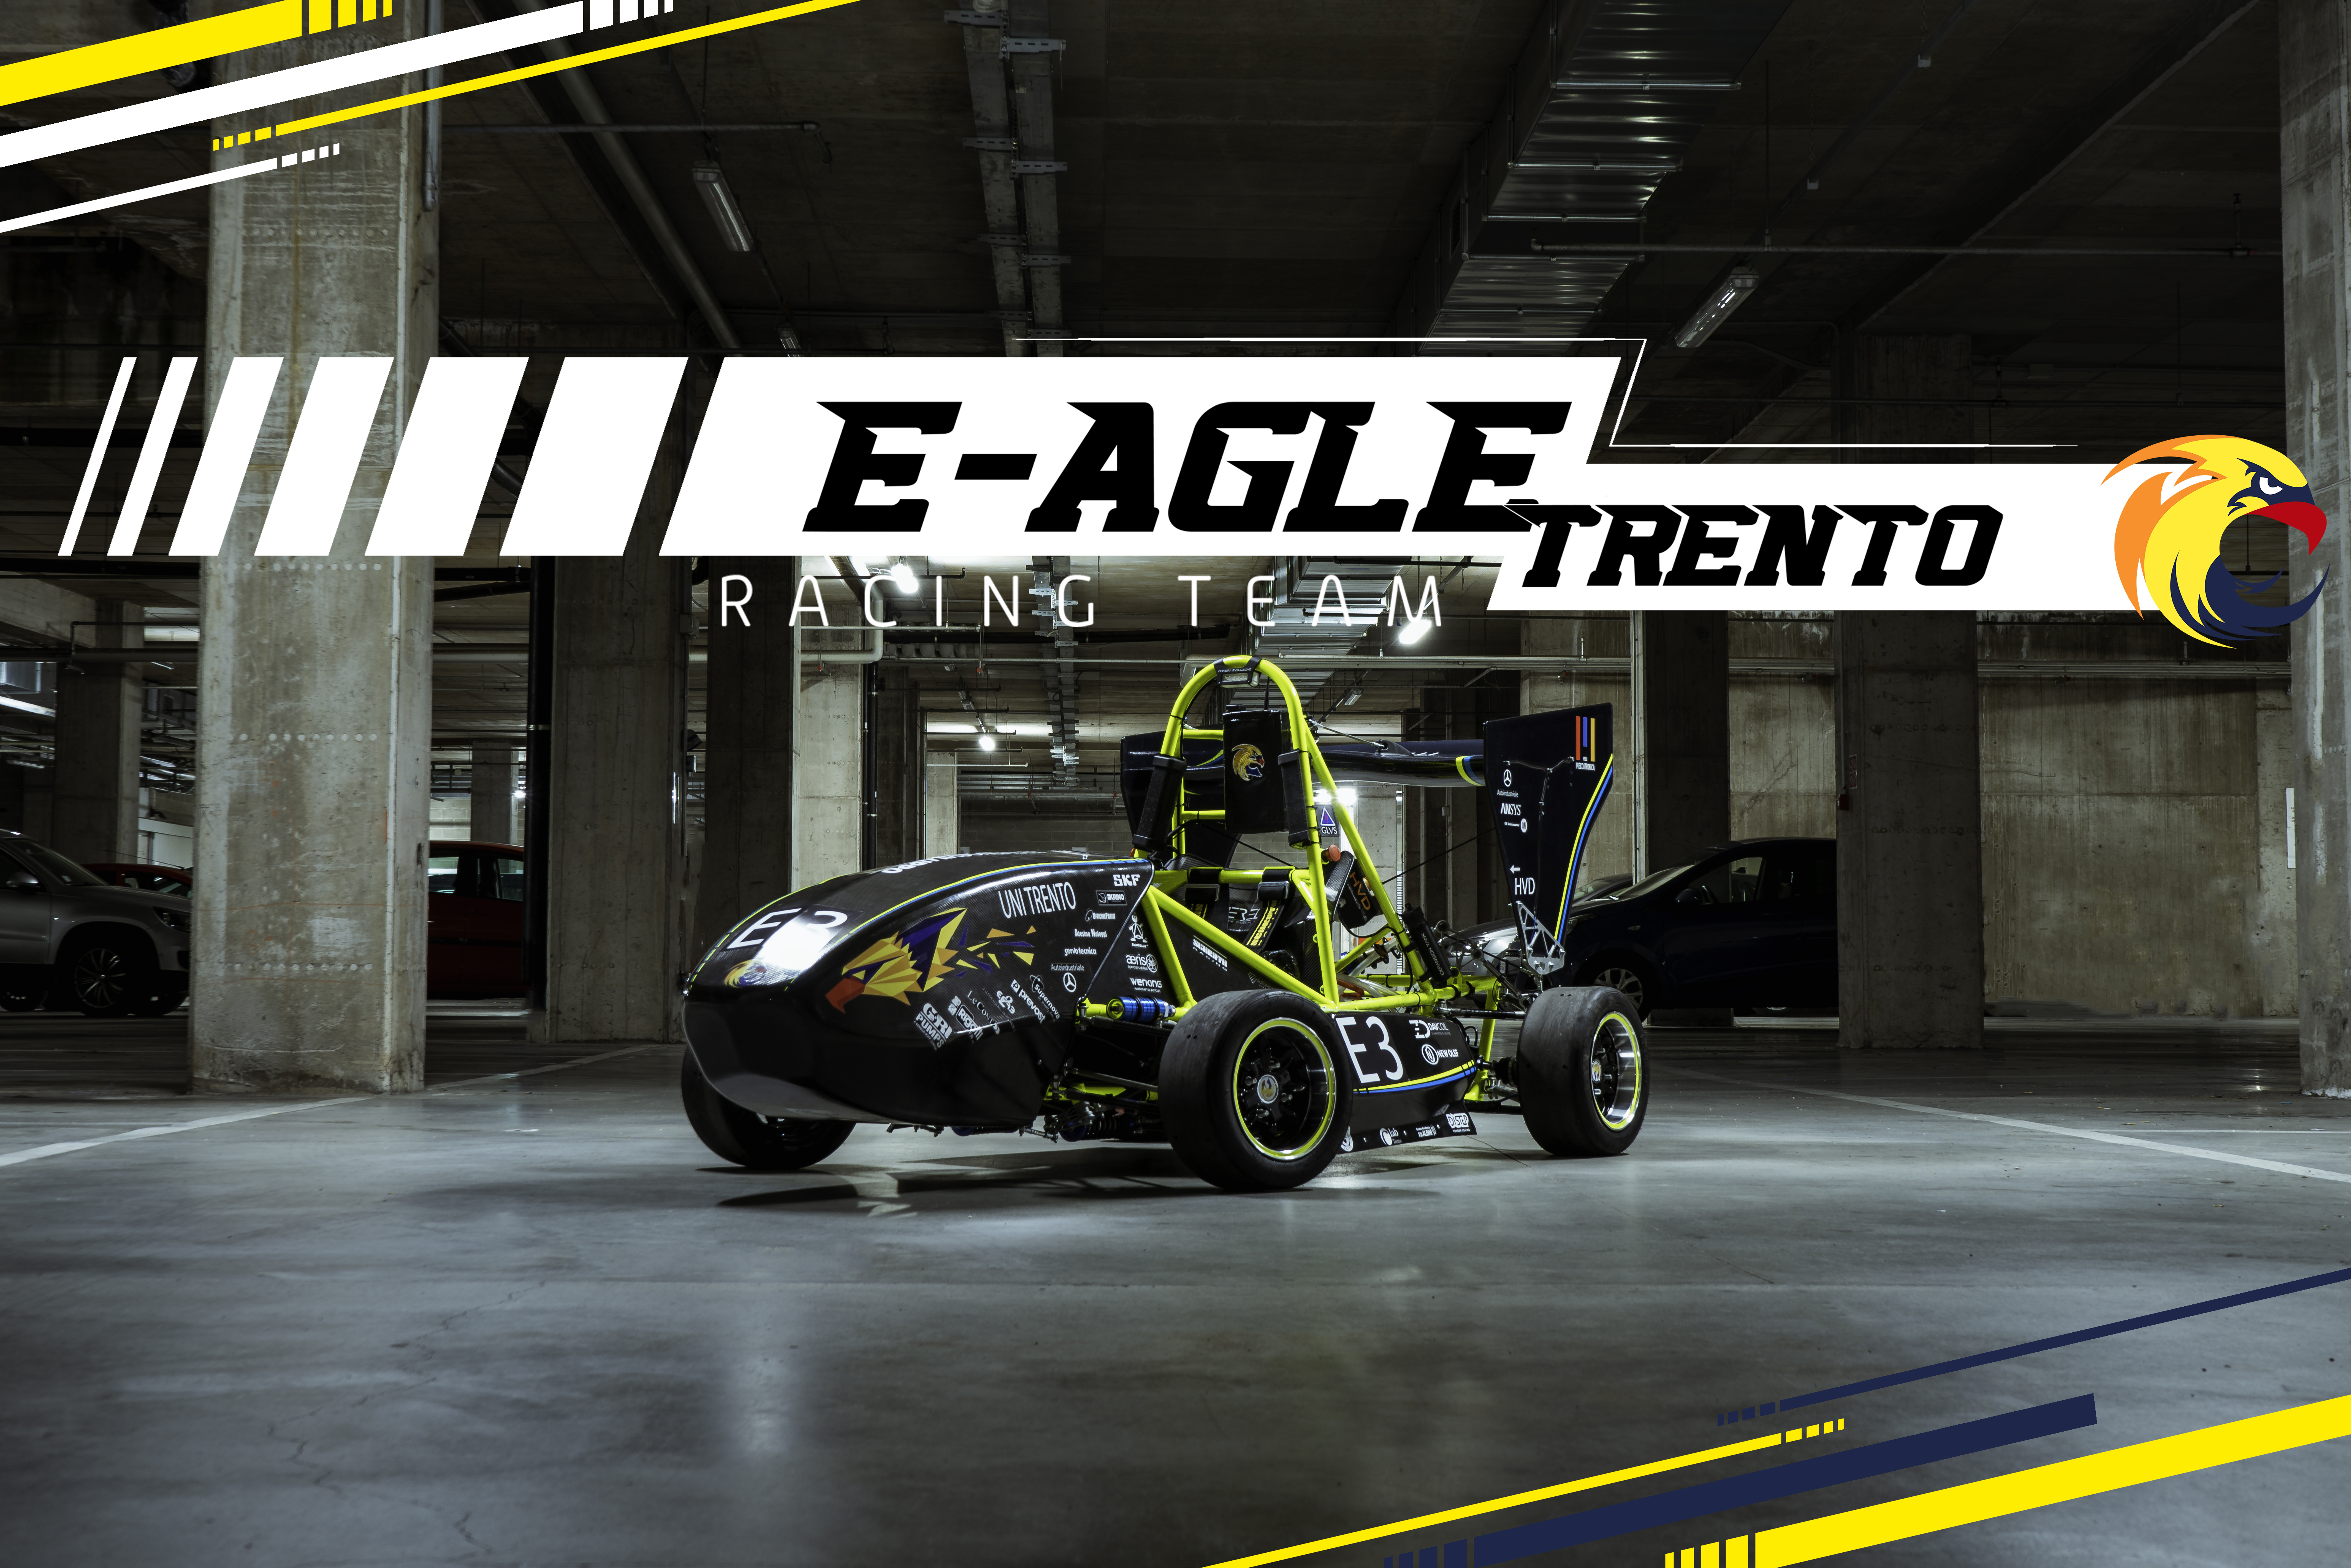
\includegraphics[width=1\textwidth]{./figures/chimera-evoluzione.jpg}
  \caption{Foto di Chimera Evoluzione}
\end{figure}

% Eagle TRT Progetto e Team
E-Agle Trento Racing Team è un'Associazione Sportiva che nasce come progetto universitario
che si occupa della progettazione, costruzione e messa in pista di un prototipo da corsa stile Formula 1 completamente elettrico. 
L'Associazione è nata nel Dicembre 2016 ed è costituita da studenti dell'Università di Trento 
dei dipartimenti di Ingegneria Industriale, Scienze Informatiche ed Economia. 
L'obiettivo principale di E-AGLE TRT è quello di competere su pista nelle competizioni organizzate dalla SAE International. 
Ad esse vi aderiscono circa 90 Università da tutto il mondo al fine di poter testare e 
dimostrare le proprie scelte tecniche e i propri risultati in termini di prestazioni, sostenibilità economica e marketing.
% Il mio Ruolo nel Team e il mio team 
Nel 2017 ho avuto l'occasione di partecipare al progetto come sviluppatore software nel gruppo Telemetria 
che si occupa di raccogliere e visualizzare i dati in real-time. 
Una parte importante del lavoro è stata condividere con gli altri membri del team 
le compteneze di ingegneria del software per poter definire una struttura per tutti gli studenti occupati nell'ambito informatico
e dare una forma alle documentazioni.
Inizialmente mi sono occupato dell'implementazione di nuove funzionalità, come la calibrazione della pedaliera direttamente dal Volante,
fino alla visualizzazione sull'interfaccia dei sensori presenti in macchina.

Questo ha permesso di rendere più stabili le funzioni principali per poi, nel secondo semestre del 2018, ridisegnare la digital dash
del Volante per facilitarne l'utilizzo, rendendolo più accativamente e migliorandone l'aggiornarnabilità.     
Tutt'ora sono impegnato come Project Manager della parte telemetrica grazie agli ottimi risultati ottenuti lo scorso anno.  

\newpage




